\documentclass[a4paper]{article}

% Pacotes para o português.
\usepackage[brazilian]{babel}
\usepackage[utf8]{inputenc}
\usepackage[T1]{fontenc}

\usepackage{sbc-template}

\usepackage{datetime}
\usepackage{graphicx}
\usepackage{float}
\usepackage{indentfirst}
\usepackage{amssymb}
\usepackage{multirow}
\usepackage[nottoc]{tocbibind}

% Espaçamento duplo.
\usepackage{setspace}
 % Breaklines nas citações.
\usepackage{cite}

% Linha horizontal.
\newcommand{\HRule}{\rule{\linewidth}{0.5mm}}
\newcommand{\hRule}{\rule{4.5cm}{0.1mm}}

% Listagens.
\newfloat{program}{thp}{lop}
\floatname{program}{Listagem}

% Figuras.
\newcommand{\figurex}[5]
{
\begin{figure}[htb, h!]
   	\setlength{\unitlength}{1.0cm}
   	\centering
   	\includegraphics[scale=#1]{./img/#2.#3}
	\begin{center}
	   	\parbox{.9\linewidth}{\footnotesize \sf \caption{#5}  \label{#4}}
	\end{center}
\end{figure}
}

\newcommand{\ck}[0]
{
\checkmark
}

\hyphenation{}

\begin{document}

%\doublespacing
\onehalfspacing

\begin{titlepage}
\begin{center}

% Topo 1.
\textsc{\Large UNIVERSIDADE FEDERAL DE ITAJUBÁ\\
	INSTITUTO DE MATEMÁTICA E COMPUTAÇÃO}\\[0.7cm]

% Topo 2.
\textsc{DEPARTAMENTO DE MATEMÁTICA E COMPUTAÇÃO}\\[2.8cm]

% Título.
\textsc{\Large Seminário}\\
\HRule \\[0.4cm]
{\Large \bfseries Arquitetura Peer to Peer}
\HRule \\[0.4cm]
\textsc{REDES DE COMPUTADORES}\\[2.8cm]

% Etc.
\begin{minipage}{0.4\textwidth}
\begin{flushleft} \large
\emph{Alunos:}\\[0.43cm]
%\hRule\\
David Mateus Batista\\
Gabriel Erzinger Dousseau\\
Gabriel Augusto Alves Taets\\
Mauricio Ferreira Leite\\
\end{flushleft}
\end{minipage}
\begin{minipage}{0.4\textwidth}
\begin{flushright} \large
\emph{Professor:}\\[0.4cm]
%\hRule\\
Bruno Guazzelli Batista
\end{flushright}
\end{minipage}

\vfill

\today

\end{center}
\end{titlepage}

\thispagestyle{empty}

\section*{Resumo}
Esta monografia tem o objetivo de estudar e analisar a arquitetura de redes Peer-to-peer,
suas vantagens, desvantagens, limitações e aplicações.
\newpage
\pagenumbering{Roman}

\tableofcontents
\newpage
\pagenumbering{arabic}

%http://www.fio.edu.br/manualtcc/co/1_Estrutura_do_TCC.html%
\section{Introdução}
\newpage

\section{Fundamentação Teórica}
\textit{Peer-to-Peer} significa, em tradução literal, "par a par". Em termos formais, os dispositivos da rede estão conectados por uma cadeia descentralizada, onde cada um possui funções equivalentes, sem hierarquias. Todos os usuários são clientes e servidores, funcionando de forma independente e livre da existência de um servidor central. A busca por um arquivo é enviada a todos os dispositivos da rede, os quais tomam conhecimentos dos outros usuários através de um hospedeiro (que apenas monitora pontos de presença na rede e não tem um banco de dados com nomes de usuários ou arquivos), que informa o IP dos usuários ativos na rede. O pedido é repassado para todos os usuários, que vão passando, usuário por usuário, até que o arquivo desejado seja encontrado.\cite{sisp2p}

É preciso notar que P2P e arquiteturas centralizadas não são alternativas disjuntas. Existem muitos sistemas que podem ser classificados como uma mistura de um sistema P2P e um sistema centralizado. O problema é que não existe uma fronteira clara entre um paradigma P2P e outros paradigmas supostamete opostos como cliente-servidor. Nos extremos, algumas arquiteturas são claramente P2P enquanto outras são claramente cliente-servidor. No entanto, existem arquiteturas que podem ser consideradas uma ou outra ou ambos, dependendo da definição de P2P considerada. Consequentemente, é importante entender o que é comum a todas as definições de P2P e o que são traços não-comuns que alguns autores incluem em suas próprias definições.\cite{camarillop2parch}

Considera-se um sistema P2P se os elementos que formam o sistema compartilham seus recursos com o propósito de prover o serviço que o sistema foi desenhado para prover. Os elementos no sistema tanto provêem os serviços aos outros elementos, como requisitam os serviços aos outros elementos. A princípio, todos os elementos no sistema devem satisfazer este critério para que o sistema seja considerado P2P. No entanto, na prática, o sistema pode ter algumas exceções (isto é, alguns nós que não satisfazem este critério) e ainda ser considerado P2P. Por exemplo, um sistema P2P pode ainda ser considerado P2P mesmo se tiver um servidor centralizado de registros. Por outro lado, alguns sistemas dividem \textit{endpoints} entre pares e clientes. Pares requisitam e oferecem serviços, enquanto clientes geralmente apenas requisitam serviços. Um sistema onde a maioria dos \textit{endpoints} se comportam como clientes não pode ser considerado estritamente P2P. \cite{camarillop2parch}

Alguns autores adicionam ainda que os elementos que foramm os sistemas P2P (que não surpreendentemente são denonimados \textit{pares}), devem ser capazes de se comunicarem diretamente, sem passar por intermediários \cite{schollmeier2001}. Outros autores dizem que o sistema deve ser auto-organizável e ter controle decentralizado\cite{roussopoulos2004}.

É notável que as definições acima são dadas no contexto de um único serviço individual. Um serviço complexo pode ser composto de vários serviços individuais. Alguns desses serviços individuais pode consistir de serviços P2P e alguns deles podem consistir de serviços cliente-servidor. Por exemplo, um cliente de compartilhamento de arquivos pode incluir um cliente P2P para efetuar o compartilhamento em si, e um navegador \textit{web} para acessar informações adicionais num servidor \textit{web} centralizado. Adicionalmente, existem arquiteturas onde um sistema cliente-servidor pode servir como "estepe" para um serviço normalmente provido por um sistema P2P, ou vice-versa. \cite{camarillop2parch}

Prover um serviço geralmente envolve processamento ou armazenamento de dados. De acordo com a definição de Camarillo, num sistema P2P, os pares compartilham suas capacidades de processamento e armazenamento (isto é, seus recursos de software e hardware), de forma que o sistema possa prover o serviço. Por exemplo, se o serviço a ser provido é um serivço de distribuição de arquivos, pares diferentes entre o sistema irão armazenar arquivos diferentes. Quando um certo par quer um arquivo em particular, primeiro ele deve descobrir qual par possui (ou quais pares possuem) o arquivo, e então obter o arquivo destes pares\cite{camarillop2parch}. Esta definição de P2P nos fornece um critério para decidir se um sistema é ou não P2P.


\begin{figure}[!ht]
\begin{center}
  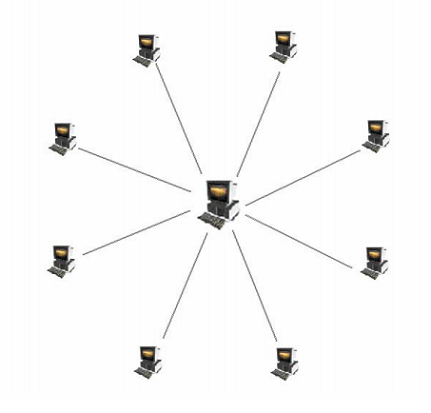
\includegraphics{img//cliente-servidor.png}
  \caption{Esquema Cliente-Servidor\cite{sisp2p}} 
\end{center}
\end{figure}

\begin{figure}
\begin{center}
  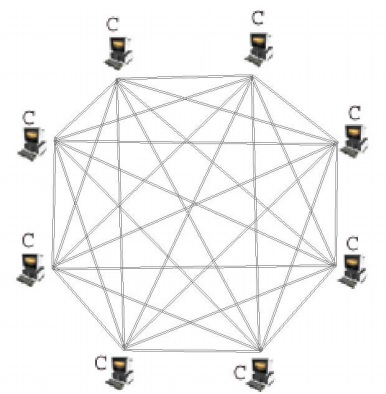
\includegraphics{img//p2p.png}
  \caption{Esquema P2P \cite{sisp2p}} 
\end{center}
\end{figure}

\begin{figure}
\begin{center}
  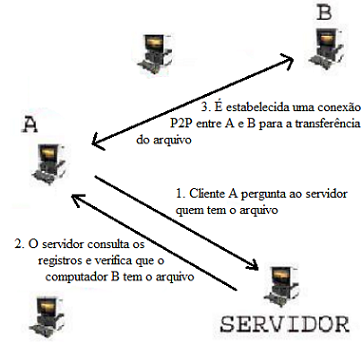
\includegraphics{img//misto.png}
  \caption{Esquema Misto \cite{sisp2p}} 
\end{center}
\end{figure}

\newpage

\section{Aplicações}
Como visto nas seções anteriores, a utilização da arquitetura \textbf{P2P} pode trazer diversas vantagens, desvantagens e outras características únicas para o aplicativo ( ou serviço ) que estará implementando-a. \\
Dessa forma, é importante analisar quais serviços utilizam essa arquitetura, como se beneficiam de suas vantagens e como lidam com suas desvantagens. Isto é, dissecar sobre como as caracteristicas da arquitetura P2P são tratadas em cada caso de uso.
\subsection{Napster}
O \textbf{Napster} foi uma das primeiras aplicações de compartilhamento de arquivos, elaborada em Junho de 1999. O serviço permitia apenas o compartilhamento de arquivos \textbf{MP3} e é um grande responsável pela popularidade do termo "P2P".
A rede se basea num servidor central de indices. Os nós da rede registram uma lista dos arquivos que desejam compartilhar. Dessa forma, a busca é processada baseando-se em \textbf{palavras chave} e retornará uma lista com os arquivos encontrados e informações como a banda disponivel, tamanho e fonte. 
\begin{figure}[!h]
\begin{center}
  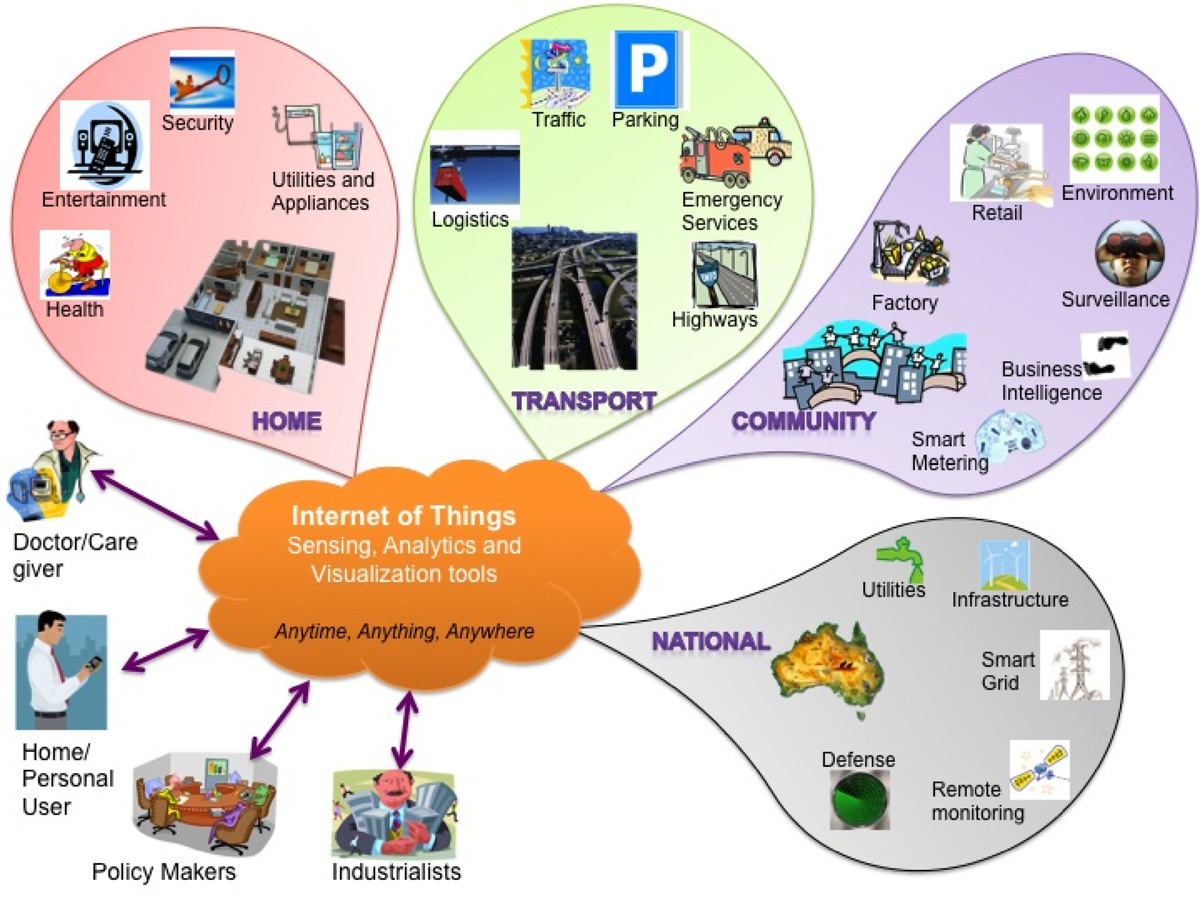
\includegraphics{img//ilustracaoiot.png} 
  \caption{Protocolo Napster \cite{?} \label{figure1}}
\end{center}
\end{figure}

A imagem acima representa o funcionamento do protocolo Napster, indicando um cliente fazendo uma \textbf{consulta} ao servidor central, para que o servidor então busque os outros clientes que possuem tal arquivo. Em seguida, tais clientes se conectam ao requisitante, para transferir o arquivo.

\subsubsection{Vantagens e Desvantagens}
Como um dos pioneiros na área, a principal vantagem do Napster se devia ao fato de ele possuir uma busca rápida e eficiente ( por se tratar apenas de uma consulta ao servidor central ). Além disso, oferecia uma visão simples e consistente da rede. \
As desvantagens se devem exatamente a \textbf{presença de um servidor}, uma vez que, assim como em arquiteturas cliente-servidor, a central representa um ponto de falha único, que se fosse afetado, prejudicaria toda a rede. Por se tratar de um servidor que lida com diversas requisições, o servidor central também possuia um alto custo de manutenção.

\subsection{Gnutella} %https://pdfs.semanticscholar.org/f0b5/86bda8901c2f3ae399b48239690028f69417.pdf
%https://pt.slideshare.net/uschmidt/peertopeer-systems/7-P2P_Filesharing_The_most_popular
Gnutella é um \textbf{protocolo de busca} aberto e descentralizado usado principalmente para o compartilhamento e a busca de arquivos. Foi criado com o objetivo de ser uma rede dinamica que permite que seus usúarios entrem e saiam a qualquer momento, tenha uma boa escalabilidade, garanta a anonimidade  e confiança em relação a ataques externos. \\
O termo Gnutella se refere a todo o grupo de computadores que possuem aplicativos carregados com o protocolo Gnutella que formam uma espécie de rede virtual. Cada nó nessa rede pode funcionar tanto como um cliente como quanto um servidor. \\
Dessa forma, eles podem criar e receber requisições com outros nós utilizando os dados que estarão em seu disco rígido. Como é sábido, tais requisições não são enviados para nenhum servidor central, elas são exclusivamente tratadas entre os nós da rede.


\begin{figure}[!h]
\begin{center}
  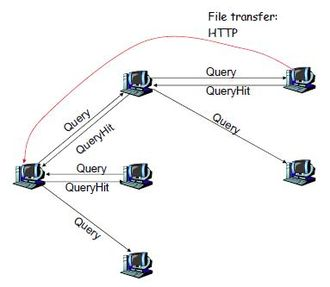
\includegraphics{img//gnuquery.JPG} 
  \caption{Protocolo Gnutella \cite{?} \label{figure1}}
\end{center}
\end{figure}

A imagem acima, representa um grupo de computadores utilizando aplicativos com o protocolo Gnutella. Na mesma, um computador realiza uma \textbf{query} buscando um arquivo nos nós da rede. Os computadores que possuirem tal arquivo, retornam um \textbf{Query hit} para que, em seguida, seja estabelecida uma conexão \textbf{HTTP} entre eles para a transmissão do arquivo. \\



\subsubsection{Mecanismo de Busca}
O protocolo utiliza o algoritmo padrão conhecido como BFS( \textbf{B}readth \textbf{F}irst \textbf{S}earch) - Busca em Largura - portanto, tal qual o algoritmo é utilizado em grafos, ele será utilizado na rede de aplicativos que utilizam o protocolo:
\begin{itemize}
	\item O nó inicialmente busca um arquivo e envia a mensagem de busca a seus vizinhos
	\item Os vizinhos encaminham a mensagem para todos os seus vizinhos
	\item Os Nós que possuirem o arquivo que está sendo requisitado, começam uma mensagem de resposta
	item Após a mensagem de resposta atingir o nó origem, o download do arquivo começa.
\end{itemize}
\subsubsection{Vantagens e Desvantagens}
O protocolo GNutella apresenta algumas modificações que \textbf{superam} as desvantagens do Napster, como por exemplo: não depender de um servidor para indexar os arquivos, dessa forma, não se cria um "único ponto de falha" na arquitetura. Entretanto, este mesmo fato causa uma das suas principais desvantagens: a busca em largura acaba por adicionar um certo periodo de tempo bem maior do que se fosse utilizado um servidor. \newline
As outras desvantagens do Gnutella possuem origem nas desvantagens da própria arquitetura P2P :  segurança, poucos usúarios servindo arquivos e perca de banda.


\newpage

\section{Discussão}
\newpage

\section{Considerações finais}
\newpage


\newpage
\bibliographystyle{plain}

\bibliography{document}


\end{document}
